\chapter{Knowledge Discovery and Data Mining}\label{chapter:kdd}

\section{Motivation}
Before we talk about the opportunities and advantages of running data mining algorithms in HyPer, we first clarify the term Data Mining. Data Mining ,also known as knowledge discovery from databases (KDD), is the process of gaining knowledge and insight from data. As already mentioned, data growth is exploding and petabytes of new data are generated every day by every aspect of daily life, such as businesses, society, science and medicine. With this huge amount of data available, data has become a very valuable resource in our decade. Data is seen as the new oil, others call data the new currency. 
These quotes highlight the importance of data. However, it is important to note that we have to transform data into knowledge to actually gain value. For example, online shopping companies like amazon are very keen to find out not only what customers bought in the past, but also what they are likely to buy in the future. Therefore, amazon is using data mining techniques to present their users products related to products they recently viewed or bought. Also products of other customers with similar interests are displayed, as shown in figure 1. In that case, data mining is used to boost the consumerism. Additionally, this knowledge can be used to optimize storage cost, e.g. by knowing how much of certain products will be sold in the next time.
Another example is Google Trends...
Other areas


\section{Knowledge Discovery}

After understanding the importance of data mining for gaining knowledge and using this knowledge for further decision making, this section defines data mining steps in greater detail. The term data mining itself often leads to confusion - we are not mining data but instead we are looking for knowledge and interesting patterns in a given data set or database. Therefore, the term knowledge discovery from databases, or KDD is not as arbitrary as data mining.


\begin{figure}[htsb]
  \centering
  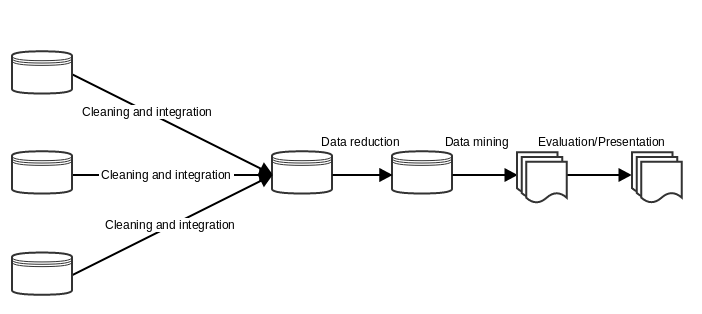
\includegraphics[scale=0.5]{figures/kdd}
  \caption[kdd]{KDD.}\label{fig:kdd}
\end{figure}

Often, data mining is seen as a part of the knowledge discovery process, as depicted by figure xx. The knowledge discovery process starts with the preprocessing steps data cleaning, integration, selection and transformation. The actual knowledge gain is then acquired in the data mining step, afterwards the knowledge is evaluated and presented. 
Regarding all those steps, Han et al. give a very accurate definition of data mining: 

“Data mining is the process of discovering interesting patterns and knowledge from large amounts of data. The data sources can include databases, data warehouses, the Web, other information repositories, or data that are streamed into the system dynamically.”
 
 In the following, we look at each of the knowledge discovery steps.




\subsection{Data Cleaning}

The first step of knowledge discovery needs to ensure that the data to be mined is complete, clean and consistent. Real world data is usually none of it. Data sets are incomplete, i.e. values are missing. Are these missing values crucial for the further data mining process, several data cleaning techniques exist to fill the gaps in the data, e.g. by using an average value such as the mean or median.
The same is true for inconsistent or redundant data. An example for inconsistent data are distinct values with the same meaning, e.g. the chars w and f both meaning female. Additionally, we often see random error or variance in a measured variable. For proper data analysis, we have to clean this noisy data first e.g. by smoothing the data set, using binning techniques.


\subsection{Data Integration}

Data mining requires often data from several sources. These sources can be databases, data warehouses, transactional data but also more complex data sets such as time-related data, data streams, spatial data, multimedia data, graph data or any data available on the Internet. All these data sources have to be integrated into one coherent data set which can be used for analysis. There are several challenges regarding data integration, the most important is the entity identification problem: When combining data from different sources same data objects can have different names and types in different schemas. Therefore, data integration often requires domain knowledge of the different data sources and techniques used in data cleaning to get a clean, consistent data source and to avoid redundancy.


\subsection{Data Reduction}

After cleaning and integrating data into a coherent data set, the data should be consistent, clean, complete and ready for further mining. However, those data sets are usually of huge size and contain much information, not all necessary for the data mining process. Data Reduction techniques can help to reduce the information density and speed up the data analysis and mining process. Simple techniques for data reduction are projection, selection and aggregation, available in every database system. More advanced techniques are dimensionality reduction, e.g. by principal component analysis, numerosity reduction above aggregation, like clustering or sampling, and data compression. 
Data transformation changes the values given data, e.g. by converting the data into another format, e.g. by using normalization. Data discretization is another part of data transformation, e.g. numeric data is presented in intervals. 
The aim of all of the addressed methods is to reduce the size of the data set to get the information the user is interested. Some methods of the presented data reduction techniques are data mining techniques as well, e.g. clustering. Therefore the line between data reduction and data mining is not always easy to draw.


\subsection{Data Mining}

After the presented steps the data sets are ready to apply actual data mining techniques. In the following sections we will revise data mining goals, techniques and the associated algorithms for frequent pattern mining, classification, clustering and outlier detection.


\subsection{Pattern Evaluation}

So far we have learned several techniques of data mining to find patterns in the data set, such as clusters, outliers or frequent item sets. We can also use training data to predict and categorize new data. 
After generating those patterns we have to evaluate them to figure out how valuable the acquired knowledge is. First, a pattern has to be understandable, e.g. a certain clustering does not gain any knowledge if the reason for it is not comprehensible. Therefore, the reasons for the clustering must be clear for the user. That leads to the next step of evaluation: A pattern has to be valid, useful and novel. Only then, a pattern can be called interesting and can be used as knowledge, e.g. by fulfilling a hypothesis the user tries to confirm. 


\subsection{Knowledge Presentation}

Knowledge presentation is then the final step of data mining. Interesting patterns have to be described and visualized to the user in an appealing, understandable format. Apart from textual explanation, several data visualization techniques exist and should be applied for the respective situation.
More ...

A section about the applicability of data mining methods in Hyper


\section{Algorithms of Data Mining}

\subsection{Mining Frequent Patterns and Association Rules}
Frequent pattern mining aims to find the most frequent items in a data set and its association rules. A typical example is the Market Basket Analysis: Supermarkets and online commercial stores are interested in what their customers are buying, in particular in items that are frequently bought together. In other words, which items are frequently put in the same market basket. 
This knowledge is very valuable: It’s not only about finding out which items are very popular, and therefore get a better a position in the market or website. It is also about knowing which items are bought together and making decisions upon this information: Related items could be placed next to each other, to make the shopping experience for the customer more convenient. Another approach would be to put related items far aways from each other, so that the customer has to walk around more in the store and is more likely to buy an additional product. That are just two possible strategies that could be applied with the knowledge of frequent pattern mining.
Most algorithms for frequent pattern mining expecting transactional data as input, because this type of data represents a market basket the best. The most popular algorithms is the Apriori algorithms, working in an iterative manner. Apriori generates itemsets of length k and checks if these itemsets appear frequent, that means if there count exceeds a given threshold. All the valid itemsets and then used in the next iteration to generate itemsets of length k+1. The algorithms converges after no more itemsets can be generated.
Since the candidate generation and the scanning of the database is expensive, there is still active research to improve the Apriori performance as well as establish other techniques. One of them is FP-growth (frequent pattern growth), an algorithm compressing the database into an FP-tree and therefore finds frequent itemsets without candidate generation. Furthermore, there exist more algorithms for more specific cases, e.g. for finding frequent patterns in high-dimensional, spatial and multimedia data.

\subsection{Classification}

n data mining, classification uses existing data as existing knowledge for predicting future events. A typical example is the identification of spam emails: Emails should be classified into two categories: spam and non-spam. This is done by labelling existing emails as spam or non-spam email. These initial set of categorized emails is then used as the training data for the classification algorithms. Based on the knowledge the algorithms gets from the training data, new emails can be classified as spam or non-spam.
Another example is to ….
Since classification needs training data, where all the data tuples have to be labelled first, classification is also called supervised learning. That means that before starting the data mining process, some previous knowledge has to be acquired. In our example, someone has to label emails first as spam or non-spam before the algorithm can be applied. 
There exist many classification algorithms in practice, the most popular ones are Naive bayes, Support Vector Machines (SVM), Decision Trees and Neural Networks.
A very popular classifier is the Support Vector Machine. An SVM requires as input training data and builds a model upon. Each data tuple is represented as a vector in the SVM model space. Since the data is labelled, the SVM knows which data tuples belong together and tries to find separating hyperplanes between them. These hyperplanes can be represented by a small subset of the data tuples, called the support vectors. This fact makes the SVM very efficient using high-dimensional data. New data tuples are then represented as a vector in the SVM space and belong the category as the other data tuples in their gap between the hyperplanes.

\subsection{Clustering}

While classification requires apriori knowledge, i.e. tuples must be labelled to be used as training data, clustering does not require any previous knowledge. In that sense, clustering is a very convenient method to gain knowledge about a data set without the need of knowing exactly what the result should look like. Therefore, clustering is also called unsupervised learning.
An example is Google News, presenting news headlines obtained from many news websites and presented in one place. There is no set of available news topics, instead the topics about what is important can change over time. Therefore, setting up training data and use classification is not feasible. Instead, clustering can be used, finding important topics in the latest news articles and groups them together. The algorithms tries to find the best grouping of news, meaning that the news objects in one group have a high similarity with each other, while they are very different to the news objects in other clusters. 
Clustering is used in all disciplines from biology, security, business intelligence and the web and comes with a wide range of algorithms. These algorithms can be categorized in the following four categories, each with advantages and disadvantages regarding the input data set.
Partitioning methods: Partitioning methods are the most popular clustering methods, trying to find clusters of spherical shape. A distance function is used to measure similarity and dissimilarity among the clusters. Most popular algorithms are k-Means and k-Medoid. 
Hierarchical methods: Hierarchical methods are useful for data consisting of several hierarchies or levels. Clustering is applied by going up or down the hierarchy tree and merging or splitting subtrees, respectively. Similar to partitioning-based methods, hierarchical cluster algorithms find spherical clusters. 
Density-based methods: Finding clusters of arbitrary shape, such as oval clusters or S shape clusters, partitioning and hierarchical methods are limited. Density-based clustering techniques obtain much better results, using dense regions in data sets for identifying clusters instead of distances from a center point. The most popular algorithms is the DBSCAN (Density-based spatial clustering of Applications with Noise) algorithm, finding core objects, i.e. objects within a dense neighbourhood and joining those core objects together to find dense regions, i.e. a cluster.
Grid-based method: All the presented methods so far are data-driven, i.e. groupings are found by the distribution of objects in the embedding space. In contrast, grid-based methods are space-driven, i.e. the object space is mapped to a finite number of cells, resulting in very fast processing times for multi-dimensional data. Popular algorithms are STING and CLIQUE. CLIQUE is a special form of grid-based algorithms, since it is both density and grid based.


\subsection{Outlier Detection}

Outlier detection are techniques to find data objects that behave in a different way than the majority of data objects. For a commercial system, outliers can be clients spending much more money than the average client. In all kind of fraud detection systems, outlier detection is very important, e.g. for medical care or security. 
Obviously, there is a strong correlation between outlier detection and clustering. Data objects that do not fit into a cluster are potential outliers, and therefore clustering techniques can be used for outlier detection. However, their main purpose is to find clusters, whereas outlier detection algorithms are specialized in finding outliers. Therefore, clustering techniques are often optimized to omit all data points in dense region and only search for outliers, leading to a more effective search.
Apart from unsupervised learning, supervised learning can be applied for outlier detection as well. First, data is labelled as normal or outlier, and therefore future data can be classified. This data is then used as training data to classify data sets as outliers or normal data. The challenge of using classification methods for outlier detection is that outliers are very rare by definition, and therefore typical classification algorithms often have to be adapted and optimized for outlier classification.
Apart from adopting clustering and classification techniques, statistical and proximity-based methods are also used for outlier detection.


